\section{Case Study}

In this section we describe a running example of our payload organ delivery system-of-system. In the example, a drone is supposed to fly over Thames River (on the water), and the wind could be favorably strong. Suppose that the original specification of a drone component did not consider these characteristics. 

According to the process in Figure~\ref{fig:process}, we first specify the scenarios of the system and component and their extensions, as shown in Section 2.2, explicitly recording global (system) and local (component) requirements.

The behaviour of the component represented in LTS is derived from the scenarios as LTS using Finite State Processes (FSP) specification language~\cite{Magee:2006:CSM:1076396}, as shown below: \\
\begin{alltt}\small
DRONE [b:Bat][d:Dis]\uwave{[o:On_Water][w:WindStrong]} =
    (takeOff -> FLYING[b-1][d]\uwave{[o][w]}),
FLYING [b:Bat][d:Dis]\uwave{[o:On_Water][w:WindStrong]} = ( 
    when (b>10 && d>0)  manoeuvre -> FLYING[b-1][d-1]\uwave{[0][0]}
  | when (b>10 && d>0)  manoeuvre -> FLYING[b-1][d-1]\uwave{[1][0]}
  | when (b>10 && d>0)  manoeuvre -> FLYING[b-1][d-1]\uwave{[0][1]}
  | when (b>10 && d>0)  manoeuvre -> FLYING[b-1][d-1]\uwave{[1][1]}
  | when (b>10 && d==0) land -> LANDING[b-1][0]\uwave{[o][w]}
  | when (b<=10 && d>0) safeLand -> LANDING[b-1][d]\uwave{[o][w]}),
LANDING [b:Bat][d:Dis]\uwave{[o:On_Water][w:WindStrong]} = (
   when (d>=0\uwave{&& o==0}) landed -> LANDING[b][d]\uwave{[o][w]}
 \uwave{\ \ | when (d>0&& o==1 && (w==1||w==0))  landed -> ERROR}).\\
\end{alltt}
\noindent where, {\it Bat} indicates percentage of the drone's battery (0..100\%) and {\it Dis} represents the remaining distance to the destination (0..5km). Note that the curly highlighted parts in the specification were not in the original component specification, they are the `joinpoints' to be matched by the pointcuts of a wrapper aspect described next.

After introducing the emerging ``On\_Water'' and ``Wind\_Strong'' domains (both ranging from 0 to 1), the specification may no longer satisfy the delivery requirement. This is due to an error in the exceptional conditions about these domains. 
% \begin{alltt}\small
% range Bat = 0..100 // in percentage
% range Dis = 0..100 // to destination
% \end{alltt}\small
%range Flying = 0..1 // boolean
%
%Then we specify the original behaviour of the drone as the following . 
%Given the situation of battery level $b>0$, distance to destination $d>0$ and not flying $f=0$, Line 2 specifies that the drone will take off from land when there is enough battery and is not at the destination, after which one unit of battery will be consumed $b'=b-1$, distance maintained $d'=d$ and flying $f'=1$.
%Similarly, Line 3 states that the drone will manoeuvre when there is battery, in the air, not at the destination; 
%Line 4 says it will land when reaching the destination, in the air, and there is still battery; Line 5 tells that it will perform `safe landing' when the battery is lower than 10\% while reaching the destination; and Line 6 considers that it has landed safely if it is not flying.
%S[b:Bat][d:Dis][f:Flying] =
% ( when (b>0 && d>0 && f==0)          takeOff -> S[b-1][d][1]
% | when (b>0 && d>0 && f==1)      manoeuvre -> S[b-1][d-1][1]
% | when (b>0 && d==0 && f==1)            land -> S[b-1][0][0]
% | when (b>0 && d>0 && f==1 && b<=10)    safeLand -> S[b-1][d][0]
% | when (f==0)                           landed -> S[b][d][0]
% ).
%\end{alltt}
%
% Line 1 declares the model name and the initial values of its internal variables: battery starts with 13\% of charge and the distance from the target hospital is 5km. Line 2 specifies that the drone will take off, after which one unit of battery will be consumed $b'=b-1$, but the distance is maintained $d'=d$. Similarly, Line 4 states that the drone will manoeuvre when the battery is above the threshold and it is not at the destination; Each manoeuvre action reduces the battery and the distance in one unit of time. 
% Line 5 says it will land when reaching the destination and there is still battery; Line 6 tells that it will perform safe landing when the battery is lower than 10\% while reaching the destination; and Line 7 considers that it has landed successfully. 
%
% \begin{alltt}\small
% S = DRONE[13][5],
% DRONE[b:Bat][d:Dis] = (takeOff -> FLYING[b-1][d]),
% FLYING[b:Bat][d:Dis] = (
%    when (b>10 && d>0)  manoeuvre -> FLYING[b-1][d-1]
%  | when (b>10 && d==0)    land -> LAND[b-1][0]
%  | when (b<=10 && d>0)    safeLand -> LAND[b-1][d]),
% LAND[b:Bat][d:Dis] = (landed -> LAND[b][d]).
% \end{alltt}
%
%
%
%\subsection{Exceptional condition}
% The exceptional condition is often visible only when additional knowledge domains are considered. For example, when the On\_Water domain is considered, the defiant component would reveal its problem as violation the global safety property. 
%
% Compared to the original specification, the following changes become visible. Line 1 indicates the same internal variable values for the previous model, but now considering that the drone is not on water initially (o==0). After taking off, lines 4 and 5 show non-determinism whether or not the drone will be on water afterwards a manoeuvre; Lines 6 and 7 remain the same, whilst Line 9 ensures that the drone is landed safely only when it is on solid ground, or it is already at the destination; Line 10 indicates that the drone will be landed unsafely if it is on the water.
%\begin{alltt}\small
%\uwave{range On\_Water = 0..1 // boolean}
%S'[b:Bat][d:Dis][f:Flying][o:On_Water] =        
%  ( when (b>0 && d>0 && f==0 && o==0) takeOff -> S'[b-1][d][1][0]
%  \uwave{| when (b>0 && d>0 && f==1)     manoeuvre -> S'[b-1][d-1][1][0]}
%  \uwave{| when (b>0 && d>0 && f==1)     manoeuvre -> S'[b-1][d-1][1][1]}
%  | when (b>0 && d==0 && f==1)           land -> S'[b-1][0][0][o]
%  | when (b>0 && d>0 && f==1 && b<=10)   land -> S'[b-1][d][0][o]
%  | when (f==0 \uwave{&& (d==0 || o==0)})        landed -> S'[b][d][0][0]
%  \uwave{| when (f==0 && d>0 && o==1)                    landed -> ERROR}
%  ).
%\end{alltt}
%% Yu: Do we want to add "b>d" to the ERROR condition?
%
Figure~\ref{fig:drone_defiant} shows an underlying LTS for the behaviour model of the drone. Note that the paths that end at states 5 or 9 indicate a trace in which the drone battery decreased to the threshold, but as it was flying over the ground (third parameter of the \textit{safeLand} action equals [0]), \textit{safeLand} is performed successfully. On the other hand, the paths reaching the error state (-1) are the ones that \textit{safeLand} was performed, but the drone was above the water, regardless of the wind strength. 

%Therefore, the exception condition is obtained as the negation of these situations that lead to the error state. 
The exceptional condition is summarised into reaching an ERROR state when the drone landed with {\tt d>0 \&\& o==1 \&\& w==1}. 
\begin{figure}
    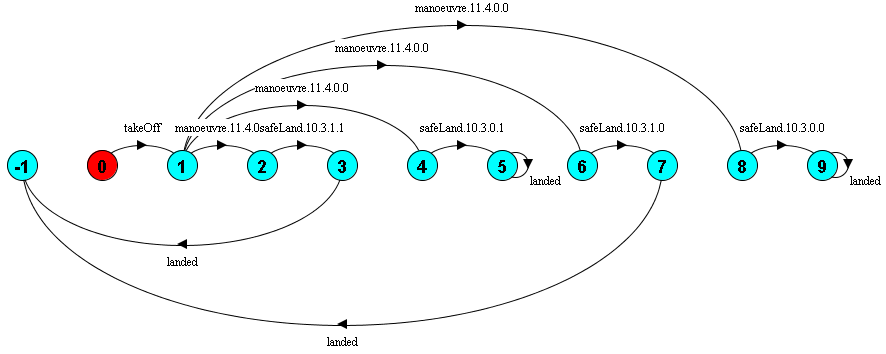
\includegraphics[width=\columnwidth]{figures/drone_defiant.png}
    \caption{LTS for the exceptional condition of the drone}
    \label{fig:drone_defiant}
\end{figure}
%
%Using the model checker of LTSA, one can get a trace, as a counter example, that violates the safety property, i.e., reaching the error state.
%
%\subsection{Aspect-oriented Adaptation: Pointcut}
%
A change request is raised. However, the component cannot be reconfigured (it is a defiant component).

To address this problem, we declare a wrapper aspect with two related parts (pointcuts and advices). {\it Pointcuts} are expressions that match with {\it join points} which can be enumerated on the specifications, i.e., the original LTS, as point of control where behaviours thereafter will be modified. {\it Advices} modifies the behaviours at the joint points to handle the exceptional conditions. 
%A wrapper aspect is defined as follows:
\hspace*{1cm}\begin{alltt}\small
{\bf aspect} WRAPPER \{
  {\bf pointcuts} \{
   ({\bf introduce}, \{o:On_Water, w:WindStrong | range 0..1\});
   ({\bf uncertain}, \{FLYING: manoeuvre\}, \{o, w\});
   ({\bf error}, \{LANDING: landed\}, \{(d>0 && o==1 && w==1)\});
  \}
  {\bf advices} \{
   ({\bf and}, \{FLYING:safeLand\}, \{(d>=2 && o==0)\});
   ({\bf opt}, \{FLYING: manoeuvre\}, \{(b<=10 && d>2 && o==1)\});
   ({\bf opt}, \{FLYING: manoeuvre->land\}, 
               \{(b<=10 && d<=2 && o==1 && w==1)\});
  \}
\}
\end{alltt}
In the pointcuts part, the `introduce' primitive adds an additional boolean domain into the declarations; the `uncertain' primitive adds the uncertainty to the post-conditions of the action of `manoeuvre'; and the `error' primitive specifies the exceptional condition on `landed' that leads to an error using the defiant component as-is. As a result, the LTS model above changes to the curly highlighted parts.

In the advices part, caution is taken so that the woven system addresses the problems of the defiant component on exceptional condition whilst maintaining expected functions for normal operations. Specifically, `and/or' primitives append AND/OR conditions to the guards, whilst `opt' primitives append new options as required by the what-if scenarios.
After weaving the wrapper, the new LTS model is presented below with its differences highlighted: (curly)\\

\begin{alltt}\small
DRONE' [b:Bat][d:Dis][o:On_Water][w:WindStrong] = 
     (takeOff -> FLYING[b-1][d][o][w]),
FLYING [b:Bat][d:Dis][o:On_Water][w:WindStrong] = (       
  when (b>10 && d>0)  manoeuvre -> FLYING[b-1][d-1]\uwave{[0][0]}
| when (b>10 && d>0)  manoeuvre -> FLYING[b-1][d-1]\uwave{[1][0]}
| when (b>10 && d>0)  manoeuvre -> FLYING[b-1][d-1]\uwave{[0][1]}
| when (b>10 && d>0)  manoeuvre -> FLYING[b-1][d-1]\uwave{[1][1]}
  | when (b>10 && d==0) land -> LANDING[b-1][0][o][w]
  | when (b<=10 && d>=2 \uwave{&& o==0})  safeLand -> LANDING[b-1][d][o][w]
  | when (b<=10 && d>2 \uwave{&& o==1)  manoeuvre ->\\ 
  LANDING[b-1][d][0][w]} 
  | when (b<=10 && d<=2 && \uwave{o==1 && w==1)  manoeuvre-> \\
  land -> LANDING[b-1][d-1][1][w])}, 
LANDING[b:Bat][d:Dis][o:On_Water][w:WindStrong] = (
  when (d>=0 && o==0) landed -> LANDING[b][d][o][w]
 | when (d>0 && o==1 && (w==1 || w==0))  landed -> ERROR).
\end{alltt}

%when (b>10 && d>0)  manoeuvre -> FLYING[b-1][d-1]\uwave{[0][0]}
%| when (b>10 && d>0)  manoeuvre -> FLYING[b-1][d-1]\uwave{[1][0]}
%| when (b>10 && d>0)  manoeuvre -> FLYING[b-1][d-1]\uwave{[0][1]}
%| when (b>10 && d>0)  manoeuvre -> FLYING[b-1][d-1]\uwave{[1][1]}
%| when (b>10 && d==0) land -> LANDING[b-1][0][o]
%| when (b<=10 && d>0 \uwave{&& (o==0||w==0)})  
%                      safeLand -> LANDING[b-1][d][o][0]),
%LANDING [b:Bat][d:Dis][o:On_Water][w:WindStrong]=(
%  when (d>0 && o==0) landed -> LANDING[b][d][o][w])
%\uwave{| when (b<=10 && d>2 && o==1)  manoeuvre \\ 
%       -> FLYING[b-1][d][0][w]}
%\uwave{| when (b<=10 && d<=2 && w==1 && o==1)  manoeuvre \\
%       -> land -> LANDING[b-1][d-1][1])}
%| when (d>0&& o==1 && w==1)  landed -> ERROR).

%\begin{alltt}\small
%S''[b:Bat][d:Dis][f:Flying][o:On_Water] =        
%  ( when (b>0 && d>0 && f==0 && o==0) takeOff -> S''[b-1][d][1][0]
%  | when (b>0 && d>0 && f==1 \uwave{|| (b>d && d>0 && o==1)})
%  								  manoeuvre -> S''[b-1][d-1][1][0]
%  | when (b>0 && d>0 && f==1 \uwave{&& (o==0 || b>d && o==1)})
%  								  manoeuvre -> S''[b-1][d-1][1][1]
%  | when (b>0 && d==0 && f==1)           land -> S''[b-1][0][0][o]
%  | when (b>0 && d>0 && f==1 \uwave{&& (b<=10 && o==0 || b<d && o==1)})
%    								     land -> S''[b-1][d][0][o]
%  | when (f==0 && (d==0 || o==0))        landed -> S''[b][d][0][0]
%  | when (f==0 && d>0 && o==1 \uwave{&& b>d})        landed -> ERROR
%  ).
%\end{alltt}
 
%\subsection{Evaluation: Verify Cautious Adaptation}
All requirement properties are verified using LTSA.
%
The {\it defiance removal} properties are checked on exceptional conditions (e.g., flying above water with a strong wind the 10\% battery is sufficient to deliver payloads).
%
The {\it safety assurance} properties on existing actions are enforced. First, it disallows change to the post-conditions to preserve the function of the defiant component. %Since the wrapper will reuse the functionality of a defiant component, it is assumed that the correct function of the defiant component will still be delivered.
Second, an action (e.g., `safeLand') with restricted precondition guarantees the same behaviour. Finally, an action (e.g., `manoeuvre') with relaxed precondition needs test obligations to ensure that existing function still work in the exceptional conditions. Otherwise, the adaptation without changing the defiant component could fail. This is a limitation that could be addressed by combining test case generation approaches, for example. 
%For example, when there is battery sufficient to fly the remaining distance to the destination, the manoeuvre function will operate to the end of delivery.

